% 编译使用xelatex
\documentclass{ctexart}

\usepackage{amsmath}
\usepackage{amsfonts}
\usepackage{amssymb}
\usepackage{tabularx}
\usepackage[math]{cellspace}
\setlength\cellspacetoplimit{6pt}
\setlength\cellspacebottomlimit{6pt}

\title{信号处理原理}

\DeclareMathOperator{\CWT}{\mathbf{CWT}}
\DeclareMathOperator{\DWT}{\mathbf{DWT}}
\DeclareMathOperator{\CTFT}{\mathbf{CTFT}}
\DeclareMathOperator{\ICTFT}{\mathbf{ICTFT}}
\DeclareMathOperator{\DTFT}{\mathbf{DTFT}}
\DeclareMathOperator{\IDTFT}{\mathbf{IDTFT}}
\DeclareMathOperator{\DFT}{\mathbf{DFT}}
\DeclareMathOperator{\IDFT}{\mathbf{IDFT}}
\DeclareMathOperator{\ZT}{\mathbf{ZT}}
\DeclareMathOperator{\ENERGY}{\mathbf{ENERGY}}
\DeclareMathOperator{\POWER}{\mathbf{POWER}}
\DeclareMathOperator{\D}{\mathbf{D}}
\DeclareMathOperator{\ud}{\mathrm{d}}
\DeclareMathOperator{\Rset}{\mathbb{R}}
\DeclareMathOperator{\Cset}{\mathbb{C}}
\DeclareMathOperator{\Zset}{\mathbb{Z}}
\DeclareMathOperator{\sgn}{\mathrm{sgn}}
\DeclareMathOperator{\Sa}{\mathrm{Sa}}
\DeclareMathOperator{\Res}{\mathrm{Res}}
\DeclareMathOperator{\STFT}{\mathbf{STFT}}

% for simulating booktabs rules; so they work with vertical lines
\newlength{\Oldarrayrulewidth}
\newcommand{\Cline}[2]{
  \noalign{\global\setlength{\Oldarrayrulewidth}{\arrayrulewidth}}
  \noalign{\global\setlength{\arrayrulewidth}{#1}}\cline{#2}
  \noalign{\global\setlength{\arrayrulewidth}{\Oldarrayrulewidth}}}
\newcommand{\Hline}[1]{
  \noalign{\global\setlength{\Oldarrayrulewidth}{\arrayrulewidth}}
  \noalign{\global\setlength{\arrayrulewidth}{#1}}\hline
  \noalign{\global\setlength{\arrayrulewidth}{\Oldarrayrulewidth}}}
\newcommand{\Topline}{\Hline{0.08em}}
\newcommand{\Bottomline}{\Hline{0.08em}}
\newcommand{\Midline}{\Hline{0.05em}}
\newcommand{\CMidLine}[1]{\Cline{0.05em}{#1}}

% for formatting a row
\newcolumntype{+}{>{\global\let\currentrowstyle\relax}}
\newcolumntype{^}{>{\currentrowstyle}}
\newcommand{\rowstyle}[1]{\gdef\currentrowstyle{#1}#1\ignorespaces}

% define new stretchable column types
\newcolumntype{L}{>{\raggedright\arraybackslash}X}
\newcolumntype{R}{>{\raggedleft\arraybackslash}X}
\newcolumntype{C}{>{\centering\arraybackslash}X}

\begin{document}
\maketitle

\tableofcontents

\section{记号与定义}
\subsection{记号}
    \begin{table}[ht!]
        \centering
        \begin{tabularx}{\textwidth}{|c|L|}
            \Topline
            记号 & 解释和性质 \\ \Midline
            $u(t)$ & 单位阶跃信号\\ \Midline
            $\delta(t)$ & 单位冲激信号 $\delta(t) = \frac{1}{a} \delta(\frac{t}{a})$ \\ \Midline
            $G(t)$ & 原点单位脉冲信号, $G(t) = \begin{cases}
                1 & -\frac{1}{2} < t < \frac{1}{2}\\
                0 & \text{otherwise} \end{cases}$
                \\ \Midline
            $Sa(t$) & Sample函数, $Sa(t) = \begin{cases}
                \frac{\sin t}{t} & t \neq 0 \\
                1 & t = 0 \end{cases}$ \\ \Midline
            $\Delta_{T} (t)$ & 周期单位冲激序列, $\Delta_T(t) = \sum_{n} \delta(t - n T)$\newline
                其有特别的性质: $\int_{\Rset} f(t) \Delta_T(t) \ud t = \sum_n f(nT)$
            \\ \Midline
            $\delta(n)$ & 单位冲激序列 $\delta(n) = \begin{cases}1 & n = 0 \\ 0 & \text{otherwise}\end{cases}$ \\ \Bottomline
        \end{tabularx}
    \end{table}

\subsection{定义}
\paragraph{信号能量} 对于连续函数, $\ENERGY[f(t)] = \int_{-\infty}^{+\infty} \|f(t)\|^2 \ud t$.
    对于离散函数, $\ENERGY[x(t)] = \sum_{n = -\infty}^{\infty} \|x(n)\|^2$.
\paragraph{信号功率} 对于连续函数, $\POWER[f(t)] = \lim_{T \to \infty} \frac{1}{T} \int_{-T/2}^{+T/2} \|f(t)\|^2 \ud t$.
    对于离散函数, $\POWER[x(t)] = \lim_{N \to \infty} \frac{1}{2N + 1} \sum_{n = -N}^{N} \|x(n)\|^2$.
\subsection{其他}
    \begin{description}
        \item[Dirichlet积分] $\int_{-\infty}^{\infty} Sa(t) \ud t = \pi$
        \item[Gaussian积分] $\int_{-\infty}^{\infty} e^{-t^2} \ud t = \sqrt{\pi}$
        \item[冲激函数的筛选特性] $\int_{-\infty}^{\infty} f(t) \delta(t - t_0) = f(t_0)$
        \item[冲激函数的位移特性] $f(t) * \delta(t - t_0) = f(t - t_0)$, 注意冲激函数点乘得值, 卷积得函数
        \item[卷积的性质] 一般的卷积满足交换律, 结合律, 分配律.
        \item[不收敛的求和] $\sum_{n = -\infty}^{+\infty} e^{-j n \omega T_1} = \omega_1 \Delta_{\omega_1}(\omega)$
    \end{description}

\section{傅里叶级数}
\subsection{三角函数形式的傅里叶级数}
    性质足够良好的周期函数都可以表达为\[
        f(t) = a_0 + \sum_{n = 1}^{\infty} \left( a_n \cos n\omega t \,+\, b_n \sin n\omega t \right)\]
    其中$T$为函数的周期, $\omega = \frac{2\pi}{T}$.
\paragraph{求解系数}
    要求$n, m \in \Zset^+$, 则函数基性质为\begin{eqnarray*}
        \int_0^{T} \sin nt\, \sin mt \ud t &=& \delta_{nm} \frac{T}{2}\\
        \int_0^{T} \cos nt\, \cos mt \ud t &=& \delta_{nm} \frac{T}{2} \\
        \int_0^{T} \sin nt\, \cos mt \ud t &=& 0
    \end{eqnarray*}
    直接由函数基性质\begin{align*}
        a_0 &= \frac{1}{T} \int_T f(t) \ud t\\
        a_n &= \frac{2}{T} \int_T f(t) \cos n\omega t \,\ud t\\
        b_n &= \frac{2}{T} \int_T f(t) \sin n\omega t \,\ud t
    \end{align*}
\subsection{复数形式的傅里叶级数}
    性质足够良好的周期函数都可以表达为\[
        f(t) = \sum_{n = -\infty}^{\infty} F_n e^{j n \omega t}
    \]其中$T$为函数的周期, $\omega = \frac{2\pi}{T}$.\par
    注意这里指数没有负号, 与傅里叶变换中形式不同.
\paragraph{求解系数}
    利用函数基性质 \[
        \int_T e^{j n \omega t} e^{j (-m) \omega t} \ud t = T \delta_{nm}\]
    有\[
        F_n = \frac{1}{T} \int_T f(t) e^{-j n \omega t} \ud t\]

\section{CTFT}
\subsection{定义}
    注意信号的傅里叶变换不一定存在. 本课程中不考虑不存在的情况.
\paragraph{对于非周期信号} $f(t)$的CTFT定义为 \[
    \CTFT[f(t)] = F(\omega) = \int_{-\infty}^{+\infty} f(t)\; e^{-j \omega t} \ud t \]
可以看成$f(t)$和基函数$e^{j \omega t}$的内积.\footnote{这里内积是酉空间内积, 需满足共轭交换}\par
    逆变换定义为 \[
    \ICTFT[F(\omega)] = f(t) = \frac{1}{2\pi} \int_{-\infty}^{+\infty} f(t)\; e^{j \omega t} \ud t \]

\paragraph{对于周期信号}
    设周期为$T_1$, 周期信号$f$的单周期截断是$f_0$, 显然$f = f_0 * \Delta_T$,
    则有 \[
        \CTFT[ f(t) ] = \omega_1 \Delta_{\omega_1}(\omega) \CTFT[ f_0(t) ] ,\quad \omega_1 = \frac{2\pi}{T_1}  \]

    \begin{table}[ht!]
    \begin{tabularx}{\textwidth}{|>{\bfseries}r  L|}
        \Topline
        线性性          & $\displaystyle \CTFT[\alpha f + \beta g] = \alpha \CTFT[f] + \beta \CTFT[g]$\\
        唯一性          & $\displaystyle \ICTFT[ \, \CTFT[f(t)] ] = f(t)$,
                            由此有$\displaystyle \ICTFT = \frac{1}{2\pi} \mathbf{R} \cdot \CTFT$\\
        对偶性          & $\displaystyle \CTFT [ \, \CTFT[ f(t) ] ] = 2 \pi f(-t)$, $\displaystyle \CTFT [ F(\nu) ] = f(-t)$
                            特别注意最后的负号\\
        反褶            & $\displaystyle \CTFT[f(-t)] = F(-\omega)$\\
        共轭            & $\displaystyle \CTFT[f^*(t)] = F^*(-\omega)$\\
        压阔            & $\displaystyle \CTFT[f(at)] = \frac{1}{|a|} F(\frac{\omega}{a})$\\
        时移            & $\displaystyle \CTFT[f(t + \tau)] = F(\omega) e^{j \omega \tau}$\\
        频移            & $\displaystyle \CTFT[f(t) e^{j \omega_0 t}] = F(\omega - \omega_0)$\\
        微分            & $\displaystyle \CTFT[\D f(t)] = j \omega F(\omega)$ \newline
                            $\CTFT[-j \omega f(t)] = \D F(\omega)$\\
        卷积            & $\displaystyle \CTFT[f g] = \frac{1}{2\pi} \CTFT[f] * \CTFT[g]$\newline
                            $\CTFT[f * g] = \CTFT[f] \CTFT[g]$\\
        和FS的关系      & $f(t)$是周期为$T_1$的函数, 傅里叶级数为$f(t) = \sum_n F_n e^{j n \omega_1 t}$,
            则$F_0(n\omega_1) = T_1 F_n$, 且$F(\omega) = \sum_n 2\pi F_n \delta(\omega - n \omega_1)$\\
        \Bottomline
    \end{tabularx}
    \caption{CTFT的性质}
    \end{table}

    \begin{table}[ht!]
        \centering
        \begin{tabular}{|c|c|}
                \hline $\displaystyle f(t)$ & $\displaystyle F(\omega)$ \\ \hline
                $\displaystyle e^{-at}\,u(t),\quad a > 0$ & $\displaystyle \frac{1}{a + j \omega}$ \\ \hline
                $\displaystyle e^{at}\,u(t),\quad a \in \Rset$ & 不存在 \\ \hline
                $\displaystyle e^{j \omega_0 t},\quad a \in \Rset$ & $\displaystyle 2 \pi \delta(\omega - \omega_0)$ \\ \hline
                $\displaystyle G(t)$ & $\displaystyle Sa(\omega / 2)$ \\ \hline
                $\displaystyle \delta(t)$ & $\displaystyle 1$ \\ \hline
                $\displaystyle 1$ & $\displaystyle 2\pi \delta(\omega)$ \\ \hline
                $\displaystyle u(t)$ & $\displaystyle \pi\delta(\omega) + \frac{1}{j\omega}$ \\ \hline
                $\displaystyle \cos (\omega_0 t)$ & $\displaystyle \pi \delta(\omega - \omega_0) + \pi \delta(\omega + \omega_0)$ \\ \hline
                $\displaystyle \sin (\omega_0 t)$ & $\displaystyle j \pi \delta(\omega + \omega_0) - j \pi \delta(\omega - \omega_0)$ \\ \hline
                $\displaystyle \Delta_{T_1} (t)$ & $\displaystyle \omega_1 \Delta_{\omega_1}(\omega),\quad \omega_1 = \frac{2\pi}{T_1}$ \\ \hline
                $\displaystyle e^{j \omega_0 t} [\alpha \le t < \beta]$ & $\displaystyle \frac{e^{j(\omega_0 - \omega)\beta} - e^{j(\omega_0-\omega)\alpha}}{j (\omega_0 - \omega)}$ \\ \hline
                $\displaystyle \sgn(t)$ & $\displaystyle \frac{2}{j\omega}$\\\hline
                $\displaystyle \frac{1}{t}$ & $\displaystyle -j \pi \sgn(\omega)$\\\hline
                $\displaystyle \Sa(t)$ & $\displaystyle \pi G \left( \frac{\omega}{2} \right) $\\ \hline
        \end{tabular}
        \caption{常见函数的CTFT}
    \end{table}

\subsection{抽样信号}
\paragraph{抽样过程} 自然地, 采用冲激串抽样 $f_S(T) = f(t)\cdot \Delta_{T_S}(t)$
\paragraph{抽样后傅里叶变换} $\displaystyle F_S(\omega) = \CTFT[ f_S(t) ] = \frac{1}{T_S} \sum_n F(\omega - n \omega_S)$.
    可以看出, 信号经过$T_S$抽样之后, 其CTFT变成一个周期为$\omega_S$的周期函数.
\paragraph{抽样定理} 对于截止频率为$\omega_c$的信号$f(t)$, 若$\omega_S \ge 2 \omega_c$, 则$F_S$是周期为$\omega_S$的函数,
    并且$\forall \omega \in [-\frac{\omega_S}{2}, \frac{\omega_S}{2}]\;:\;F_S(\omega) = \frac{1}{T_S} F(\omega)$. 其中$2\omega_c$称为Nyquist频率.


\clearpage


\section{DTFT}
\subsection{前置定理}
\paragraph{抽样离散定理} 由定义可证下式
    \[F_S(\omega) = \sum_{n=-\infty}^{\infty} f(nT_S) e^{- j \omega n T_S}\]过程如下
    \begin{align*}
        F_S(\omega) &= \int_{-\infty}^{\infty} f(t) \cdot \Delta_{T_S}(t) \cdot e^{-j \omega t} \ud t\\
            &= \int_{-\infty}^{\infty} f(t) \cdot e^{-j \omega t} \cdot \Delta_{T_S}(t) \ud t\\
            &= \sum_{n=-\infty}^{\infty} f(nT_S) e^{-j \omega nT_S}
    \end{align*}
    可以看成是一种抽样近似的思想, 因为在Nyquist区间内, 有\begin{eqnarray*}
        F(\omega) &=& \frac{1}{T_S} F_S(\omega)\\
        \int_{-\infty}^{+\infty} f(t) e^{-j \omega t} \ud t &=& \frac{1}{T_S} \sum_{n = -\infty}^{+\infty} f(nT_S) e^{-j \omega nT_S}
    \end{eqnarray*}

\subsection{定义} $x(n)$为频率/时间归一化的信号, $x(n) = f(nT_S)$, 则有\[
    \DTFT[x(n)] = \sum_{n = -\infty}^{+\infty} x(n) e^{-j \omega n} \]
    并且定义逆变换为 \[
    \IDTFT[X(\omega)] = \frac{1}{2\pi} \int_{-\pi}^{\pi} X(\omega) e^{j \omega n} \ud \omega\]

\subsection{时间/频率归一化}
    CTFT处理, $f(t), F(\omega)$中的$t, \omega$是物理空间中的时间/频率, 称为模拟时间/频率.
    DTFT中, 以上定义中$x(n), X(\omega)$中的$n, \omega$是数字时间/频率.\par
    数字时间用$n$表示, 范围是整数集$\Zset$, 而模拟时间$t$的范围是实数集$\Rset$.
    数字 (角) 频率的范围是一个Nyquist区间$[0, 2\pi)$, 而模拟频率的范围也是整个实数集$\Rset$.\par
    当且仅当完成无损采样的情况下, 数字时间/频率才有意义.
    数字时间$n$, 数字频率$\omega_D$, 模拟时间$t$和模拟频率$\omega_A$的关系如下式.
    \begin{eqnarray*}
        n        & \Rightarrow & t = n T_S                      \\
        t        & \Rightarrow & n =
            \begin{cases} \frac{t}{T_S} & \frac{t}{T_S} \in \Zset \\ \text{undefined} & \text{otherwise (not on sampled point)} \end{cases}\\
        \omega_A & \Rightarrow & \omega_D = \frac{\omega_A}{\omega_S} 2\pi \\
        \omega_D & \Rightarrow & \omega_A = \frac{\omega_D}{2 \pi} \omega_S
    \end{eqnarray*}

    上式中$T_S$是符合Nyquist要求的采样周期, $\omega_S = \frac{2\pi}{T_S}$.
    可以看出, 数字时间的范围是离散的$\Zset$.

    \begin{table}[ht!]
    \begin{tabularx}{\textwidth}{|>{\bfseries}r  L|}
        \Topline
        和CTFT关系 & $\displaystyle \DTFT[x](\omega) = \CTFT[f_S](\frac{\omega}{T_S})$
            如果采样频率在Nyquist区间内, 则有 $X(\omega) = \frac{1}{T_S} F\left(\frac{\omega}{T_S}\right)$\\
        线性性 & $\displaystyle \DTFT[\alpha x + \beta y] = \alpha \DTFT[x] + \beta \DTFT[y]$\\
        周期性 & $\displaystyle X(\omega + 2\pi) = X(\omega)$\\
        反褶 & $\displaystyle \DTFT[x(-n)] = X(-\omega)$\\
        共轭 & $\displaystyle \DTFT[x^*(n)] = X^*(-\omega)$\\
        压扩 & $\displaystyle \DTFT[x(n/a)] = X(a\omega), \quad a \in \Zset$\\
        时移 & $\displaystyle \DTFT[x(n + n_0)] = X(\omega) e^{j \omega n_0}$\\
        频移 & $\displaystyle \DTFT[x(n) e^{j \omega_0 n}] = X(\omega - \omega_0)$\\
        微分 & $\displaystyle \DTFT[nx(n)] = j \D X(\omega)$\\
        卷积 & $\displaystyle \DTFT[x * y] = X Y,\quad \DTFT[x y] = \frac{1}{2\pi} X * Y$
            其中的卷积$X * Y$是周期函数的卷积$\int_{-pi}^{\pi} X(\vartheta) Y(\omega - \vartheta) \ud \vartheta$\\
        能量 & $\displaystyle \ENERGY[x] = \frac{1}{2\pi} \ENERGY[DTFT[x]]$, 亦称Parseval定理\\
        \Bottomline
    \end{tabularx}
    \caption{DTFT的性质}
    \end{table}

\clearpage

\section{DFT}
\subsection{定义}
    数字信号$x$是长度为$L$的信号$x(0), x(1) \ldots x(L - 1)$,
    考虑$X = \DTFT[x]$在$\omega_k$上的值$X(\omega_k)$. 其中
    $\omega_0 = 0, \omega_1 = \frac{2\pi}{N} \ldots \omega_{N - 1} = \frac{(N-1) \cdot 2\pi}{N}$
    是Nyquist区间$[0, 2\pi)$上均匀分布的$N$个频率. 这样即得到DFT的定义
    \[
        X(k) = X(\omega_k) = \DFT[x(n)] = \sum_{n = 0}^{L - 1} x(n) W_N^{nk},\quad 0 \le k \le N - 1\]
    称为其N点DFT. 其中$W_N$是$N$次单位根\emph{倒数}$W_N = e^{- j \frac{2 \pi}{N}}$.\par
    另外定义其逆变换IDFT为\[
        \hat{x}(n) = \frac{1}{N} \sum_{k = 0}^{N - 1} X(k) W_N^{-nk},\quad 0 \le n  \le N -1 \]

\subsection{补零和回绕} 对于$L \neq N$的$x(n)$, 可以通过补零和回绕, 得到一个$L = N$的$\hat{x}(n)$, 满足$\hat{X}(k) = X(k)$.
    注意补零和回绕只会改变$L$.
\paragraph{补零} 如果$L < N$, 考虑$\hat{x}(n) = \begin{cases} x(n) & 0 \le n \le L - 1\\ 0 & otherwise \end{cases}$
\paragraph{回绕} 如果$L > N$, 考虑$\hat{x}(n) = \begin{cases} \sum_m x(n + mN) & 0 \le n \le N - 1 \\ 0 & otherwise \end{cases}$\par
    由定义, 从IDFT只能得到回绕序列$\hat{x}$, 即DFT不满足唯一性 $\IDFT[\DFT [x]] \neq x$. 但是在$N = L$的情况下, DFT仍然满足唯一性.
\paragraph{信号在时间上的约定}
    归一化情况下, 对于$n < 0$或者$n \ge L$, $x(n)$的取值有多种约定 \begin{enumerate}
        \item $x(n) = x(n \mod L),\quad n < 0, n \ge L$
        \item $x(n) = 0,\quad n < 0, n \ge L$
        \item $x(n)$未定义$,\quad n < 0, n \ge L$
    \end{enumerate}
    不同的作者, 不同的上下文会选择不同的约定.

\subsection{性质}
    基本与DTFT性质相同. 另外容易看出, 可以使用矩阵乘法计算DFT.\par
    \begin{table}[ht!]
    \begin{tabularx}{\textwidth}{|>{\bfseries}r  L|}
        \Topline
        和DTFT的关系 &  $\DFT[x](k) = \DTFT[x](\frac{k}{N} 2\pi)$\newline
                        注意DTFT参数是有限长的$x(n),\;n\in[0, L)$\newline
                        而不是通常的$f(nT_S),\;n\in\Zset$ \\
        和CTFT的关系 &  如果采样符合Nyquist频率, 则有\newline
                        $X(k) \approx \frac{1}{T_S} \CTFT[f] (\frac{k}{N} \omega_S)$ \newline
                        其中$f$是原函数, $f_{0\ldots LT_S}$是$f$截断到区间$[0, LT_S)$的函数, 
                        $x(n) = f(nT_S)$, 不是严格等于因为加窗的引入的误差  \\
        线性性 &  $\displaystyle \DFT[\alpha x + \beta y] = \alpha \DFT[x] + \beta \DFT[y]$    \\
        周期性 &  $\displaystyle X(k + N) = X(k)$    \\
        对偶性 &  $\displaystyle \DFT[X(k)] = N x(-n)$    \\
        反褶 &  $\displaystyle \DFT[x(-n)] = X(-k)$    \\
        共轭 &  $\displaystyle \DFT[x^*(n)] = X^*(-k)$    \\
        时移 &  $\displaystyle \DFT[x(n + m)] = X(k) W_N^{km}$    \\
        频移 &  $\displaystyle \DFT[x(n) W_N^{nm}] = X(k + m)$    \\
        卷积 &  $\displaystyle \DFT[x * y] = X Y$\newline
                $\DFT[x y] = \frac{1}{N} X * Y$\newline
                其中的卷积$X * Y$是周期函数的卷积$\sum_{m = 0}^{N-1} X(m) Y(n-m)$   \\
        能量 &  $\displaystyle \ENERGY[x] = \frac{1}{N} \ENERGY[\DFT[x]]$, 亦称Parseval定理\\
        \Bottomline
    \end{tabularx}
    \caption{DFT的性质}
    \end{table}

\subsection{例子}
    以下均假设DFT为N点DFT.
    \begin{table}[ht!]
    \centering
    \begin{tabularx}{\textwidth}{|CC|}
            \Topline $\displaystyle x(n)$ & $\displaystyle X(k)$ \\ \Midline
            $\displaystyle G_N(n)$ & $\displaystyle N\delta(k) = \begin{cases} N & k = 0\\ 0 & \text{otherwise}\end{cases}$
            \\
            \Bottomline
    \end{tabularx}
    \caption{DFT的例子}
    \end{table}

\subsection{FFT}
    设$N = 2N'$, 令$y(n) = x(2n), z(n) = x(2n+1),\quad 0 \le n \le N' - 1$, 则有\[
        \DFT_{N} [x] = \DFT_{N'} [y] + W_N^k \DFT_{N'} [z] \]
    按照此原理, 容易得到$\Theta(n \lg n)$的DFT算法, 而按定义计算是$\Theta(n^2)$的.

\section{STFT}
\subsection{时变信号} 从物理的角度, 一个信号在不同时间包含的分量是不同的.
    如开来的火车笛声, 最开始是较高, 之后变低.
    因此需要考虑信号在某个时间点/段的频域表示, 然而传统CTFT只在整个$\Rset$上考虑.
\subsection{STFT}
    对于时变信号$f(t)$, 定义其STFT为\[
        \STFT[f(t)] = F(\tau, \omega) = \int_{-\infty}^{+\infty} f(t) w(t - \tau) e^{-j\omega t} \ud t\]
    其中$w(t)$是窗函数.
    课程中不知为何积分中是$w^*$, 本应是先将$f(t)$加窗之后再和傅里叶基求内积的.
    因此为了自然这里稍有改动.
\paragraph{窗函数相关} 显然窗函数$w$需要满足的性质是,
    只在一个小区间$[-t_0, t_0]$中的值足够大, 此区间外都可以看成$0$.
    这个区间的长度称为窗口大小.\par
    显然, 窗口越小, 时间分辨率越好 i.e. $F(\tau, \omega)$越能反映在$\tau$这个点而不是其附近一片的性质;
    窗口越大, 频率分辨率越好.\par
    窗函数可以选择矩形窗函数, 但更常选择Gaussian窗$w(t) = e^{-\frac{t^2}{2 \sigma^2}}$
\paragraph{和原始CTFT的关系} 显然有下式. 从中看出, STFT事实上就是信号加窗的CTFT.
    \[ \STFT[f(t)](\tau, \omega) = \CTFT[f(t)w(\tau-t)](\omega)\]

\section{Wavelet Transform}
\subsection{基本思想}
\subsubsection{背景}
    STFT的问题是, 窗函数是固定的 i.e. 窗口大小不能变化.
    即, 时间分辨率/频率分辨率不能变.\par
    而考虑现实情况, 比如人对于一个频率范围内的声音最敏感.
    如同样的声高变化, 在1000 Hz左右比在15000 Hz左右更容易被察觉.
    即, 在1000 Hz 左右, 人耳的频率分辨率更高.\par
    因此需要对于不同频率-时间点, 有不同的分辨率.
\subsubsection{小波定义}
    称$\psi(t)$为小波基函数, 或小波母函数, 当且仅当
    \[ \int_{-\infty}^{+\infty} \psi(t) \ud t = 0 
        \quad\land\quad
        \ENERGY[\psi(t)] < \infty \]
\paragraph{小波基的时移和压扩}
    单个小波基类似于$e^{j\omega_0 t}$, 只包含频率信息.
    为了让其包含时间和窗口大小信息, 实际使用的基是$
        \psi_{s\tau}(t) = \frac{1}{\sqrt{s}} \psi\left(\frac{t-\tau}{s}\right) $\par
    可以看出, 时移用于确定时间; 压阔用于控制在这个时间-频率点上, 窗函数的大小;
    而$\frac{1}{\sqrt{s}}$用来使得能量不变.
\subsubsection{连续小波变换}
    类似所有的基分解思想, $f(t)$与基$\psi_{s\tau}(t)$内积得到分量值, 如下式所示
    \[
        \CWT[f(t), \psi(t)](s, \tau) = \int_{-\infty}^{+\infty} f(t) \psi^*_{s\tau}(t) \ud t
    \]
    其中频域信息$\omega$被包含在了$\psi(t)$中.

\section{系统}
\subsection{基本概念}
\paragraph{理解}
    一般的看法是, 信号进入一个系统, 然后出来后变成另一个信号. 即, 系统对信号做了一个变换.
    因此, 系统可以看作一个信号域上的算子.\par
    以$\mathcal{F}, \mathcal{G}\ldots$记系统.\par
    滤波器也是系统, 但是着重强调其对于系统在频域上的变换.
\paragraph{课程限制}
    课程中只考虑离散时间系统, 信号的时域是离散的.
    即信号域是$x(n) \in \Cset,\; x\in \Zset$, 输入输出信号都是这种形式.
    滤波器也是数字滤波器, 频域只考虑一个Nyquist区间$[0, 2\pi)$或者$[-\pi, \pi)$.\par
    并且都满足线性性, 时不变性, 因果性.\par
    另外假设输入$x$满足因果性, 即$x(n) = 0, \;\forall\, n < 0$.
\paragraph{其他概念}
    \begin{description}
        \item[线性性] $\mathcal{F}[\alpha x + \beta y] = \alpha \mathcal{F}[x] + \beta \mathcal{F}[y]$
        \item[时不变性] $\mathcal{F}[x(n + m)](k) = \mathcal{F}[x(n)](k + m)$
        \item[因果性] $y = \mathcal{F}[x]$, 则$y(n)$是$\{ x(k) \;|\; k \le n \}$的函数
        \item[稳定性] $y = \mathcal{F}[x]$, 若$x$是有界的, 则$y$是有界的.\\
                i.e. $\|x\|_{\infty} < \infty \Rightarrow \|y\|_{\infty} < \infty$
    \end{description}
    课程考虑的系统必定满足 线性性, 时不变性, 因果性. 如不考虑$x(n) \to x^2(n)$.

\subsection{时域描述}
\subsubsection{差分方程}
    $y = \mathcal{F}[x]$由以下方程确定 \[
        \sum_{k = 0}^N a_k y(n - k)  = \sum_{k = 0}^M b_k x(n - k)\]
    称如上的系统为$N$阶滤波器.
\subsubsection{流图}
    有三种单元: 延时单元, 加法单元, 乘法单元. 如图\ref{sys-unit-graph}所示.
    \begin{figure*}[ht!]
    \centering
    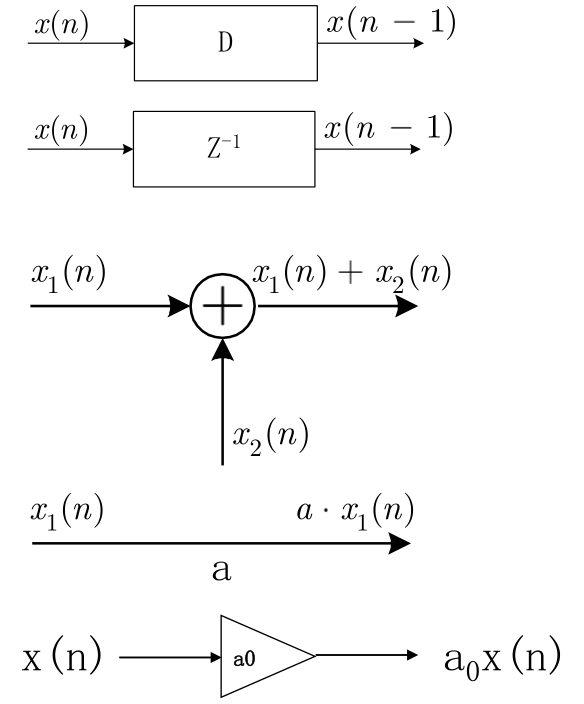
\includegraphics[width=0.6\textwidth]{sys-unit-graph.png}
    \caption{三种流图单元}
    \label{sys-unit-graph}
    \end{figure*}
\paragraph{构建方法} \begin{itemize}
        \item 直接I型构建法. 简单明白.
        \item 级联滤波器. 减少延时单元的深度, 降低因过深的延时单元链造成的指数级误差.
        \item 直接II型构建法. 减少了对输入和输出状态的存储, 即延时单元减少.
    \end{itemize}注意图\ref{dir-1}和图\ref{dir-2}中$a_k, b_k$和差分方程中的$a_k, b_k$定义不同. 下图中, 是\[
        y(n) = \sum_{k = 0}^M a_k x(n-k) + \sum_{k = 1}^{N} b_k y(n-k)\]
    \begin{figure}[ht!]
    \centering
    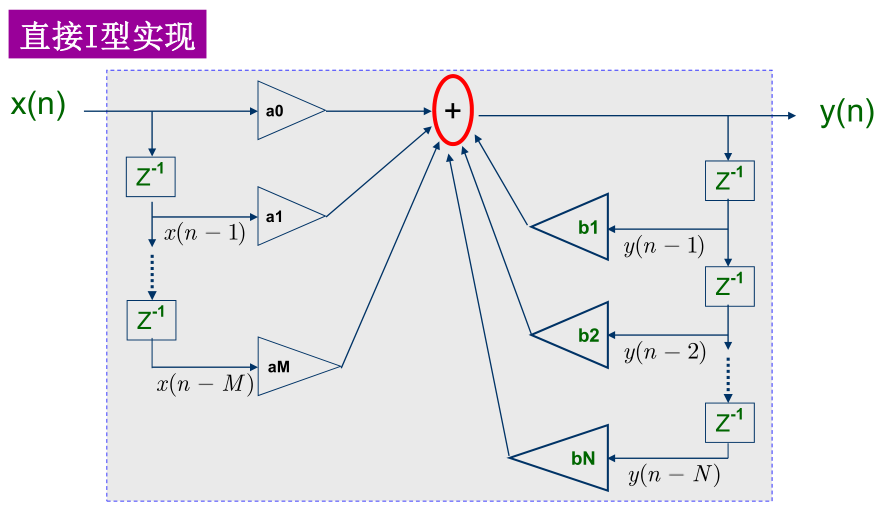
\includegraphics[width=0.95\textwidth]{dir-1.png}
    \caption{直接I型}
    \label{dir-1}
    \end{figure}
    \begin{figure}[ht!]
    \centering
    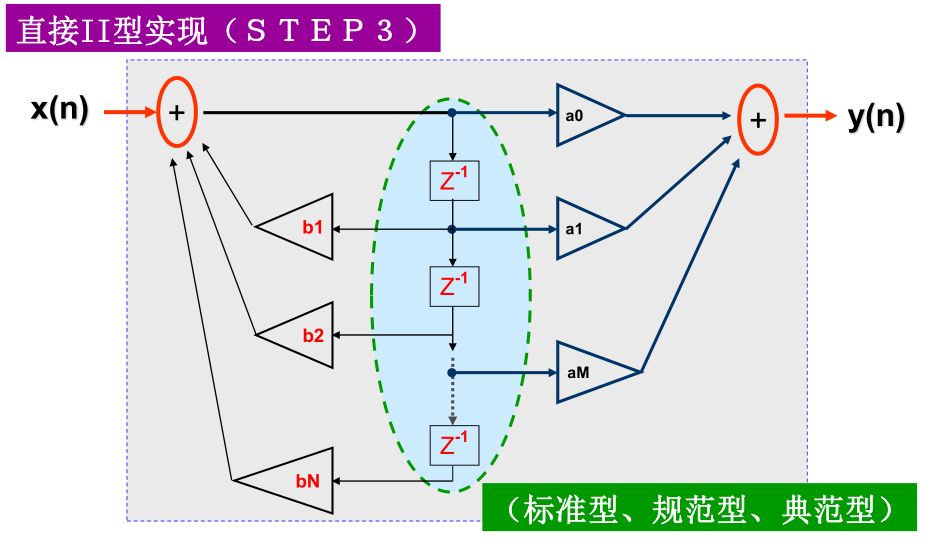
\includegraphics[width=0.95\textwidth]{dir-2.png}
    \caption{直接II型}
    \label{dir-2}
    \end{figure}

\subsubsection{冲激响应}
    $\mathcal{F}[\delta(n)]$称为$\mathcal{F}$的冲激响应 (Impluse Response).
    根据冲激响应是否在有限时间内收敛到$0$, 也分为有限和无限冲激响应.\par
    记$h(n) = \mathcal{F}[\delta]$, 因为$x(n) = \sum_k x(k) \delta(n - k) = x * \delta$,
    故不严谨地有,
    \begin{align*}
        \mathcal{F}\left[x\right] &= \mathcal{F}\left[x * \delta\right] \\
        &= \mathcal{F}\left[\sum_k x(k)\delta(n - k)\right]\\
        &= \sum_k x(k) \mathcal{F}\left[\delta(n - k)\right]\\
        &= \sum_k x(k) h(n - k)\\
        &= x * \mathcal{F}\left[\delta\right]
    \end{align*}
\paragraph{应用} \begin{description}
        \item[稳定定理] $\sum_n |h(n)|$绝对收敛 $\Leftrightarrow$ $\mathcal{F}$是稳定系统.
        \item[串联] 设$\mathcal{F}[\delta] = h_{\mathcal{F}},\,\mathcal{G}[\delta] = h_{\mathcal{G}}$,
            则$\mathcal{F} \mathcal{G} [\delta] = h_{\mathcal{G}}  * h_{\mathcal{F}} $
        \item[并联] $\left(\mathcal{F} + \mathcal{G}\right) [\delta] = h_{\mathcal{F}} + h_{\mathcal{G}}$
    \end{description}

\subsection{频域描述}
    以下频域描述都采用DTFT而非CTFT.
\subsubsection{定义} $X = \DTFT[x]$是信号的频域表示, $Y = \mathcal{F}[X]$,
    则定义$H(\omega) = \frac{X(\omega)}{Y(\omega)}$为滤波器的频率响应.\par
    其中将$|H(\omega)|$称为幅频响应, $\arg H(\omega)$称为相频响应.
\paragraph{和冲激响应的关系} 对$y = x * h$两边DTFT得到$Y = X \cdot \DTFT[h]$\\ 故有$H = \DTFT[h]$, 其满足DTFT的所有性质.

\subsection{Z变换}
\subsubsection{定义} $x(n)$是离散时域信号,
    则$x$的Z变换定义为$X(z) = \ZT[x(n)](z) = \sum_n x(n) z^{-n}$\par
    形式上类似DTFT中$e^{-jwn}$换成了$z^{-n}$, 变成了Laurent级数的形式.
    但是注意Laurent级数是$\sum_n x (n) z^n$, 而Z变换是$\sum_n x (n) z^{-n}$.
\subsubsection{收敛域} $X(z)$的收敛域 (ROC) 定义为 $\{z \;|\; X(z)\text{收敛}\}$.
    Laurent级数收敛域是一个环, 但是课程中不考虑环的边界.
\paragraph{收敛域求解} $\Omega$为Laurent级数$x(n),\,n\in\Zset$的收敛环, 则
    \[\forall z \in \mathring{\Omega}\;:\;
        \sum_n x(n)z^{-n}\;\text{收敛} \Leftrightarrow
        \sum_n x(n)z^{-n}\;\text{绝对收敛} \]
    收敛环可以通过比值法或根值法求出.
\paragraph{零-极点图}  在复平面上用$\times$表示极点,
    $O$表示零点, 画出所有零点和极点, 即得到零-极点图.
\subsection{函数空间的理解}
    可以认为, 基函数是$u_n(z) = z^{-n},\,n \in \Zset$, 由Laurent级数容易得到基函数的完备性.\par
    设$C$是任何一个以$O$为圆心的圆环, 内积定义为\begin{align*}
        \left\langle u_n(z), u_m(z) \right\rangle &= \oint_C u_n(z) u_m^*(z) z^{-1} \ud z\\
            &= \oint_C z^{-n} (z^{-m})^* z^{-1} \ud z\\
            &= \oint_C r^{-n} e^{-i \theta n} r^{-m} e^{-i \theta m} r^{-1} e^{-i \theta} \ud z\\
            &= \int_0^{2\pi} i r^{-n-m-1} e^{i \theta (m - n)} \ud \theta\\
        &= 2 \pi i r^{-n-m-1} \delta_{nm}\end{align*}
    其中假设$C$是半径为$r$的圆环, $\delta$是Kronecker delta记号.
\subsection{唯一性}
    Z变换不具有唯一/可逆性. 这一点可以从Laurent展开的非唯一性看出.
    一般地, 有如下性质:
\paragraph{Z变换级数展开}
    如果$f(z)$的极点 (即复函数的奇点) 有$N$种不同的模 (即$N=|\{|z_p|\}|$) 则存在$N+1$个不同的信号, 使得它们的ZT都是$f(z)$.
    若将其极点的模从小到大排成$\left\langle a_1, a_2\ldots a_N\right\rangle$,
    则这些信号的ROC是$\langle r1=0, r2=a_1 \rangle,\;$$\langle r1=a_1, r2=a_2\rangle\ldots$
    $\langle r1=a_N, r2=\infty\rangle$.\par
    例如, 对于$f(z) = \frac{1}{1- a^-1z}$, 显然$x(n) = a^n u(n)$和$y(n) = -a^n u(-n-1)$的ZT都是$f(z)$.
    两者的收敛域分别是$\langle r1=a, r2=\infty\rangle$和$\langle r1=0, r2=a\rangle$
\subsubsection{性质}
    \begin{center}
    \begin{tabularx}{\textwidth}{>{\bfseries}Sl  SL}
        线性性 &  $\displaystyle \ZT[\alpha x + \beta y] = \alpha \ZT[x] + \beta \ZT[y]$\\
        反褶 & $\displaystyle \ZT[x(-n)] = X(z^{-1})$\\
        共轭 & $\displaystyle \ZT[x^*(n)] = X^*(z^*)$\\
        压扩 & $\displaystyle \ZT\left[x(\frac{n}{a})\right](z) = \ZT[x](z^a)$, 其中如果$\frac{n}{a}$不是整数则$x(\frac{n}{a}) = 0$\\
        时移 & $\displaystyle \ZT[x(n + m)] = \ZT[x]z^m$\\
        频移 & $\displaystyle \ZT[a^n x(n)] = \ZT[x]\left(\frac{x}{a}\right)$\\
        卷积 & $\displaystyle \ZT[x * y] = X Y,\qquad \ZT[x y] = \frac{1}{2 \pi i} \oint X(v) \,Y\!\left( \frac{z}{v} \right) v^{-1}\ud v  $\\
        初值 & $\displaystyle x(0) = \lim_{z \to \infty} X(z)$, 当然极限不存在时此式无效\\
        终值 & $\displaystyle \lim_{n \to \infty} x(n) = \lim_{z \to 1} (z - 1) X(z)$, 当然极限不存在时此式无效\\
    \end{tabularx}
    \end{center}

    \begin{table}[ht!]
    \centering
    \begin{tabularx}{\textwidth}{|SCSCSC|}
            \Topline $\displaystyle x(n)$ & $\displaystyle X(z)$ & ROC(r1, r2) \\ \Midline
            $\displaystyle \delta(n) $ & $\displaystyle 1 $ & $\displaystyle [0, \infty]$ \\
            $\displaystyle u(n) $ & $\displaystyle \frac{1}{1 - z^{-1}}$ & $\displaystyle (1, \infty] $\\
            $\displaystyle G_N(n) $ & $\displaystyle \frac{1 - z^{-N}}{1 - z^{-1}}  $ & $\displaystyle (0, \infty] $\\
            $\displaystyle a^n $ & 不存在 & 空 \\
            $\displaystyle a^nu(n) $ & $\displaystyle \frac{1}{1 - az^{-1}}$ & $\displaystyle (\,|a|, \infty]  $\\
            %$\displaystyle   $ & $\displaystyle  $ & $\displaystyle   $\\
            \Bottomline
    \end{tabularx}
    \caption{常见信号的Z变换}
    \end{table}

\subsubsection{逆变换求解}
\paragraph{数值方法} 如果$X(z)$是有理函数, 则可以通过多项式除法来求解. 可以依次求出$x(0), x(1) \ldots$.
\paragraph{留数法} 根据留数定理, 可求得$x(n) = \sum_{z_p\text{是极点}} \Res\left[X(Z) z^{n - 1}, z_p\right]$.\
    设$z_0$是$f(z)$的$n$级极点, 则$\Res[f(z), z_0] = \frac{1}{(n-1)!} \lim_{z \to z_0} \D^{n-1} \left( (z - z_0)^n f(z) \right)$.
    可以一次得到对于一个$n$的$x(n)$.
\paragraph{有理函数展开法} 类似生成函数, 直接求根展开有理函数, 可以一次得到所有$x(n)$.
    基本原理是, 任何有理函数$R(z^{-1}) = \frac{P(z^{-1})}{Q(z^{-1})}$可以写成一个多项式和若干$\frac{T(z^{-1})}{(1-z_pz^{-1})^l}$之和,
        其中$T(z^{-1})$是多项式且$\deg T < l$, 并且$z_p$是$l$级极点.

\subsection{系统函数}
    记$X(z) = \ZT[x], Y(z) = \ZT[y]$, 则定义\[H(z) = \frac{Y(z)}{X(z)}\]称$H(z)$为系统的响应函数.\par
\paragraph{性质} 频率响应基本相同, 另有\begin{description}
        \item[因果性] $H(z)$是因果系统的充要条件是其收敛域无界, 即$r2 = \infty$
        \item[稳定性] $H(z)$是稳定系统的充要条件是其在单位圆上绝对收敛, 即$r1 < 1$
    \end{description}
\subsubsection{和差分方程的关系}
    对于差分方程描述$\sum_{k = 0}^N a_k y(n - k) = \sum_{k = 0}^M b_k x(n - k)$, 两边做ZT即有
    \[
        H(z) = \frac { \sum_{k = 0}^M b_k z^{-k}} {\sum_{k = 0}^N a_k z^{-k}}
    \]

\subsection{滤波器的设计}
\subsubsection{FIR低通滤波器的设计}
\paragraph{理想滤波器} 显然$\CTFT[\frac{\sin(t \omega_C)}{t \pi}] = G(\frac{\omega}{2\omega_C})$.
    因此在数字频率上, $\frac{\sin(n \omega_C)}{n \pi}$是一个理想滤波器,
    其中$\omega_C$是数字截止频率$\omega_C = 2\pi \frac{f_C}{f_S}$.
\paragraph{设计步骤} 基本有如下几步 \begin{enumerate}
        \item 选择$\omega_C$, 为理想滤波器的数字截止频率
        \item 计算$h(n) = \frac{\sin(n \omega_C)}{n \pi}$
        \item 根据阻带衰减, 选择窗函数
        \item 查表计算得到窗长$N$ ($N$舍入到最近奇数, $N = 2k +1$)
        \item 根据$N$计算窗函数的表达式$w(n)$
        \item FIR表达式为$h(n)w(n),\quad |n| \le k$
        \item 平移FIR, 得到因果FIR为$h(n-k)w(n-k)$
    \end{enumerate}
    FIR滤波器必定是稳定的.
\subsubsection{FIR其他滤波器}
\paragraph{高通和带通} 将低通最终得到的$h_1(n) = h(n-k)w(n-k)$移位即可$h_2(n) = h_1(n) \cos(n\omega_0)$.\par
    另外带通也可以通过低通且高通的方法实现.
\paragraph{带阻} 带足就等于低通加高通.
\subsubsection{IIR滤波器的实现}
\paragraph{双线性变换} 双线性变换将$H(s)$变为$H(z)$, 式为\[
        s = 2 f_S \frac{z-1}{z+1}\]
\paragraph{巴特沃斯滤波器}
    对于一阶, 是$H(s) = \frac{\Omega_{p1}}{s + \Omega_{p1}}$, 其中$s = j \Omega$.
    因此 $|H(\Omega)| = \frac{1}{\sqrt{\left(\frac{\Omega}{\Omega_{p1}}\right)^2 + 1}}$
\paragraph{求解步骤}
    \begin{enumerate}
        \item 根据题目写出模拟边缘频率 $f_{p1},\;f_{s1}$.
            其中$f_{p1}$是$-3 \;\textrm{dB}$的频率
        \item 计算阻带边缘增益, $\delta_S = 10^{x/20}$,
            其中$f_{s1}$的增益是$x \;\textrm{dB}$
        \item 计算得到数字边缘频率 $\omega_{p1} = 2\pi \frac{f_{p1}}{f_S}$,
            以及$\omega_{s1} = 2\pi \frac{f_{s1}}{f_S}$
        \item 用预扭曲方程求出滤波器的边缘频率
            $\Omega_{p1} = 2 f_S \tan \frac{\omega_{p1}}{2}$,
            以及
            $\Omega_{s1} = 2 f_S \tan \frac{\omega_{s1}}{2}$
        \item 根据方程\[
                n \ge \frac
                    { \lg\left(\delta_S^{-2} - 1\right)  }
                    { 2 \lg\left( \frac{\Omega_{s1}}{\Omega_{p1}}\right)} \]
            求得IIR的阶数$n$
        \item 如果$n = 1$, 利用上述一阶公式计算$H(z)$
    \end{enumerate}

\section{好题}
\paragraph{CTFT} 不用暴力求$F(\omega)$, 其中$f(t) = \begin{cases} |\sin(\pi t)| & |t| < 1\\ 0 & \text{otherwise} \end{cases}$


\pagebreak
\section{好题解析}
\paragraph{CTFT} 不用暴力求$F(\omega)$, 其中$f(t) = \begin{cases} |\sin(\pi t)| & |t| < 1\\ 0 & \text{otherwise} \end{cases}$\par
    考虑$f(t) = \sin(\pi t) \cdot \left( G(t-0.5) + -G(-t+0.5) \right)$\par
    答案是 $\left[\Sa\left(\frac{\omega - \pi}{2}\right) - \Sa\left(\frac{\omega + \pi}{2}\right)\right] \cos \frac{\omega}{2}$

\section{其他技巧}
\subsection{卷积求法}
    序列线卷积可以撕纸来求. 注意项数要足够!\par
    圆卷积的是先填零/回绕之后再求.\par
    也可采用类似乘法的方法, 例如

    \begin{table}[ht!]
        \centering
        \begin{tabular}{*{7}{c}}
        x(6) & x(5) & x(4)     & x(3) & x(2) & x(1) & x(0) \\
        \Midline
             &      &          & 1    & 2    & 3    & 4    \\
             &      & $\times$ & 4    & 3    & 2    & 1    \\
        \Midline
             &      &          & 1    & 2    & 3    & 4    \\
             &      & 2        & 4    & 6    & 8    &      \\
             & 3    & 6        & 9    & 12   &      &      \\
        4    & 8    & 12       & 16   &      &      &      \\
        \Midline
        4    & 11   & 20       & 30   & 20   & 11   & 4    \\
        \end{tabular}
        \caption{线卷积}
    \end{table}

    \begin{table}[ht!]
        \centering
        \begin{tabular}{*{7}{c}}
        x(6) & x(5) & x(4)     & x(3) & x(2)        & x(1)        & x(0)         \\
        \Midline
             &      &          & 1    & 2           & 3           & 4            \\
             &      & $\times$ & 4    & 3           & 2           & 1            \\
        \Midline
             &      &          & 1    & 2           & 3           & 4            \\
             &      & 2        & 4    & 6           & 8           &              \\
             & 3    & 6        & 9    & 12          &             &              \\
        4    & 8    & 12       & 16   &             &             &              \\
        \Midline
             &      &          & 1    & 2           & 3           & 4            \\
             &      &          & 4    & 6           & 8           & \bfseries 2  \\
             &      &          & 9    & 12          & \bfseries 3 & \bfseries 6  \\
             &      &          & 16   & \bfseries 4 & \bfseries 8 & \bfseries 12 \\
        \Midline
             &      &          & 30   & 24          & 22          & 24           \\
        \end{tabular}
        \caption{圆卷积}
    \end{table}

\end{document}
